% 学位论文 : 第二章 实验技术及设备简介
% 
% 更新记录:
%   {$LastChangedBy$}
%   {$LastChangedRevision$}
%   {$LastChangedDate$}

\chapter{GaAs/Si异变外延插入量子点位错阻挡层}
\section{背景}
量子点,为啥能解决
方案概要,量子点⇒异变外延生长

自从1982年,Arakawa从理论上计算出了当采用量子点结构作为激光器的有源区,激光器的性能将得到大幅度提升,并且由于量子点结构中不存在高能级,使得量子点激光器的阈值电流不会受到温度的影响\cite{Arakawa1982}。自此,量子点引起了众多研究者的关注。量子点主要作为激光器有源区被大家广泛研究,但是由于量子点本身会有应力,而应力层可以阻挡穿透位错的向上攀移,所以近年来也有了关于采用量子点作为位错阻挡层的报道。

对于InAs/GaAs量子点,其生长模式是SK模式,由于InAs与GaAs之间存在7\%的晶格失配,使得当InAs材料在GaAs材料表面生长时,若InAs厚度小于1ML,InAs会以点状或线状的分子集合体镶嵌在GaAs衬底中\cite{Hill1995};如果InAs生长厚度超过1ML但小于临界厚度(1.5-1.7ML),就会形成InAs/GaAs应变量子阱;而当InAs生长厚度超过临界厚度时,InAs则成岛状生长,结构为浸润层(wetting layer)上分布岛状结构\cite{Xiaoping1996}。 这种岛状结构便是量子点,其具有椎体形状或金字塔形\cite{Grundmann1995.11969}\cite{Grundmann1995.249}\cite{Cusack1996}。由于量子点是靠InAs分子应力堆积而成,量子点本身存在应力。

从理论上来说,应变层可以使得穿透位错改变方向。这个方向的改变使得部分穿透位错终止或者是穿透至样品边缘,使得穿透位错密度减少。三维量子点边缘的应变区域要比二维超晶格应变区域大很多,这就使得量子点下面的位错向上穿透会受到更大的阻力,则更容易弯曲。在GaN材料系中,通过采用腐蚀坑技术,已经证实了量子点作为位错阻挡层可以降低材料的穿透位错密度。

在该研究中,我们采用的以量子点为位错阻挡层的GaAs/Si外延片生长方案,简述如下:首先,我们在GaAs衬底上生长InAs量子点,优化量子点生长参数;以GaAs衬底量子点的生长参数为基础,进一步调节Si衬底上的量子点生长参数,在Si衬底上生长InAs单层量子点;以单层量子点为位错阻挡层,生长GaAs/Si外延片;在单层量子点的基础上,在Si衬底上生长多层量子点;以多层量子点为位错阻挡层生长GaAs/Si外延片。

从生长层中单元能量最小化方面分析,当失配大约为2\%时岛的生长模式比较好。面边缘的弹性弛豫能,面的归一化表面能和相邻岛的相互作用能是自组织生长的驱动能。总之,这些岛是共格应变和没有位错产生的,但是这些岛会部分弛豫。如果这些岛继续生长,共格生长会恶化为超过临界大小的非共格生长(弛豫生长),从而形成失配位错。


\begin{figure}[ht]
	\centering
	\includegraphics[width=0.8\textwidth]{ch05_QDbending.pdf}
	\caption{量子点阻挡$60^\circ$位错截面示意图}
	\label{fig:QDbending}
\end{figure}


如图\ref{fig:QDbending},假设自组织的岛是金字塔形,位错在晶格失配的界面形成,并向上穿透至岛的底部。位错的弯曲会形成一个失配位错环,在岛的下面滑移。弯曲发生在由于失配位错能$\Delta E_{rel}$等于或大于位错本身的能量$\Delta E_{dis}$\cite{Tillmann2000}\cite{Ovidko2002},其中$\Delta E_{rel}$和$\Delta E_{dis}$用下式表示:

\begin{equation}
	\label{eq:Erel}
	\frac{( \Delta E_{rel})}{L}=\frac{(2G_{dot} (1+v))}{(1-v)}f_{eff} b_{eff}h
\end{equation}
\begin{equation}
	\label{eq:Edis}
	\frac{( \Delta E_{dis})}{L} = \frac{1}{2\pi} \frac{G_{buff} G_{dot}}{G_{buff} + G_{dot}} b^2 (\frac{1-v\cos^2\beta}{1-v})[\ln(\frac{2r}{b}+1]
\end{equation}

公式中,L是失配位错的长度,$G_{dot}$是点的杨氏模量,$G_{buff}$是缓冲层的杨氏模量,$v$是泊松比(GaAs为0.3),$b_{eff}$是与量子点缓冲层界面相平行的伯格斯矢量,h(x,y)是以x和y为参数的量子点的高度,$\beta$是伯格斯矢量和位错线之间的角度,r(x,y)是位错应变区域的外部半径,$f_{eff}$是量子点和下面的缓冲层之间的晶格失配,假设金字塔状的量子点的宽度是W,高度是H=pW,其中p是一个几何常量,L与W成正比。Jun Yang et al \cite{NoCite}根据上式比较了InAs、InGaAs和InAlAs量子点阻挡位错的区域与量子点大小和密度的关系,结果得出大岛并且岛密度较大时,位错阻挡能力较好。

与多层应变层超晶格相似,多层量子点更适合做位错阻挡层,并且使穿透位错弯曲的能力更高。然而,当量子点层数太多,累积的应变会很大,则会形成失配位错环来释放多余的应变。多余应变的产生,主要是在于量子点层被埋没的深度,若浸润层厚度很薄则较容易发生应变过大。根据Tsao和Dodson提出的多余应力模型\cite{Tsao1988}可以估计在形成失配位错前临界量子点层数。
方程如下:

\begin{equation}
	\label{eq:tsao}
	2G_{dot} (\frac{1+\nu}{1+\nu}) \varepsilon_{eq}(z) - \frac{b}{2 \pi z \cos\beta} \frac{G_{buff} G_{dot}}{G_{buff}+G_{dot}} \times (\frac{1-\nu\cos^2\beta}{1-\nu}) [\ln⁡ \frac{4z}{b}] \geq 0 
\end{equation}

其中

\begin{equation}
	\label{eq:epsilon_eq}
	\varepsilon_{eq} (z) =  \int_0^z f_{avg}\frac{dz'}{z}  = \frac{f_{avg}h}{h+h_s}
\end{equation}

表示积累的应变。$z$是多层量子点的厚度,$h=H/3$是金字塔状量子点的有效高度,$h_s$是GaAs浸润层的厚度。为了计算积累的应变,将三维的量子点等同于厚度为$h=H/3$的二维应变层。
参数$f_{avg}$表示的是GaAs浸润层和量子点层之间的平均失配度。量子点层每个单元区域的应变能可表示为

\begin{equation}
	\label{eq:Eela}
	E_{ela} = 2G_{dot}f_{eff}^2 \frac{(1+\nu)}{(1-\nu)}(\rho_{dot}\int_{dot}{}dV)/h
\end{equation}

然而量子点的应变能还可以表示为$E_{ela}=2G_{dot}\frac{(1+\nu)}{(1-\nu)}f_{avg}^2$,失配位错$f_{avg}$可表示为

\begin{equation}
	\label{eq:f_avg}
	f_{avg} = W_{\rho_{dot}}^{\frac{1}{2}} f(1-exp(-\frac{k}{p}))^{\frac{1}{2}}
\end{equation}

其中$\rho_{dot}$是量子点密度。经计算,根据量子点岛的大小,InAs量子点的临界层数为10-15层。
由于在MBE系统中,InAs量子点的成核过程、成分组成和生长速率等方面较容易控制,使得用MBE生长的量子点均匀性和发光性能都较好,目前对于量子点作为GaAs/Si外延片位错阻挡层的研究基本都是采用MBE生长。MOCVD系统在对于速率、成分组成等方面的控制较困难,因此生长高质量的量子点具有很大的挑战性,为了进一步研究采用MOCVD技术在Si基上生长量子点,在本研究中,我们采用MOCVD系统生长InAs量子点,并以其做位错阻挡层。

\section{量子点生长}

\begin{figure}[ht]
	\centering
	\includegraphics[width=0.8\textwidth]{ch05_ThreeStep.pdf}
	\caption{三步法生长示意图}
	\label{fig:ThreeStep}
\end{figure}

在量子点生长之前,我们采用三步法生长了GaAs/Si外延片作为基础和对比样品。具体生长方案如下:

\begin{enumerate}[(1)]
	\setlength{\itemsep}{-3pt}
	\item 缓冲层:在Si衬底上,420℃条件下生长GaAs缓冲层70nm;
	\item 中间温度层:630℃条件下生长GaAs中间温度层300nm;
	\item 高温层:在中间温度层基础上以685℃生长2.7um的高温层,
	\item 退火:在高温层1.5um处插入一次三周期的热循环退火。
\end{enumerate}

经测试,该样品的FWHM=135arcsec, RMS=3.91nm

\subsection{单层量子点的生长}

\begin{figure}[ht]
	\centering
	\includegraphics[width=0.4\textwidth]{ch05_1xQD.pdf}
	\caption{单层量子点生长示意图}
	\label{fig:1xQD}
\end{figure}

经过GaAs衬底单层量子点的生长条件优化,得出GaAs衬底单层量子点的最优生长条件为:生长时间60s, V/III族比为     ,生长速率为       ;

我们采用GaAs衬底单层量子点的最优生长条件在Si衬底上生长量子点,并调节生长时间确定Si衬底上生长InAs单层量子点的最优生长条件。

首先我们在Si衬底上生长GaAs缓冲层,其中GaAs缓冲层的生长条件与2726的生长条件一致,GaAs高温层生长厚度为1.7μm,并且在高温层1.5μm处插入一次三周期热循环退火。下面是单层量子点样品的AFM测试图,其中量子点的生长时间分别为60s、65s、70s和80s。

\begin{figure}[ht]
	\centering
	\includegraphics[width=0.8\textwidth]{ch05_1xQD_AFM_10x10.pdf}
	\caption{在10um×10um扫描范围内AFM的测试图,其中量子点的生长时间分别为:a. 60s b.65s c.70s d.80s}
	\label{fig:1xQD_AFM_10x10}
\end{figure}

\begin{figure}[ht]
	\centering
	\includegraphics[width=0.8\textwidth]{ch05_1xQD_AFM_2x2.pdf}
	\caption{在2um×2um扫描范围内AFM的测试图,其中量子点的生长时间分别为:a. 60s b.65s c.70s d.80s}
	\label{fig:1xQD_AFM_2x2}
\end{figure}

从两图(图\ref{fig:1xQD_AFM_10x10}和图\ref{fig:1xQD_AFM_2x2})可以看出,当量子点生长时间为60s(这是GaAs衬底上量子点的最优生长条件)时,量子点密度很低,无大岛出现;当量子点生长时间为65s时,量子点沿原子台阶生长,量子点大小、密度均匀,基本无大岛产生;当量子点生长时间为70s时,量子点密度较大,且有大岛出现;当量子点生长时间为80s时,量子点密度很大,且大岛密度也很大。大岛团簇外延GaAs会导致位错的产生,使得位错密度增大,因此,量子点位错阻挡层要抑制大岛的产生。

\subsection{多层量子点的生长}

\begin{figure}[ht]
	\centering
	\includegraphics[width=0.4\textwidth]{ch05_3xQD.pdf}
	\caption{三层量子点生长示意图}
	\label{fig:3xQD}
\end{figure}

在单层量子点的基础上,我们研究了Si衬底上生长多层InAs量子点(如图\ref{fig:3xQD})。首先是在Si衬底上生长三层量子点,Si衬底与InAs量子点之间GaAs缓冲层的生长条件与单层量子点中GaAs缓冲层的生长条件一致。我们分别生长了65s和70s三层InAs量子点。量子点的测试结果如图\ref{fig:3xQD_AFM_30nm}所示。

\begin{figure}[ht]
	\centering
	\includegraphics[width=0.8\textwidth]{ch05_3xQD_AFM_30nm.pdf}
	\caption{图(a)(b)分别为10um×10um范围内,70s和65s三层量子点的AFM图;图(c)(d)分别为2um×2um范围内,70s和65s三层量子点的AFM图;}
	\label{fig:3xQD_AFM_30nm}
\end{figure}

由上图可以看出,生长三层量子点之后,量子点密度和大岛团簇的密度变大,70s量子点生长较65s量子点生长恶化更加严重。我们怀疑是间隔层太薄,导致量子点应力积累,使得大岛团簇增加。为了探究产生该现象的原因,我们在量子点生长时间为70s的基础上又加厚了间隔层的生长厚度,将间隔层的厚度从30nm增加到60nm。该样品的AFM测试结果如图\ref{fig:3xQD_AFM_60nm}。

\begin{figure}[ht]
	\centering
	\includegraphics[width=0.8\textwidth]{ch05_3xQD_AFM_60nm.pdf}
	\caption{10um×10um范围内,70s和65s三层量子点的AFM图}
	\label{fig:3xQD_AFM_60nm}
\end{figure}

由图\ref{fig:3xQD_AFM_60nm}可以看出,大岛团簇的密度并没有减少,所以排除了间隔层厚度的影响。所以我们认为在Si衬底上生长多层量子点,由于量子点单层所产生的应力无处释放,多层量子点生长会导致应力积累,从而导致多层量子点大岛团簇的增加。在接下来的生长中,我们采用间隔层为30nm生长多层量子点。

\begin{figure}[ht]
	\centering
	\includegraphics[width=0.4\textwidth]{ch05_5xQD.pdf}
	\caption{五层量子点生长示意图}
	\label{fig:5xQD}
\end{figure}

在量子点三层生长的基础上,我们又进行了五层量子点的生长,如图\ref{fig:5xQD}。我们认为65s生长的三层量子点密度较大,且大岛团簇较少,所以选择65s作为五层量子点中单层量子点的生长时间。测试结果如下:

\begin{figure}[ht]
	\centering
	\includegraphics[width=0.8\textwidth]{ch05_5xQD_AFM.pdf}
	\caption{五层量子点的AFM图}
	\label{fig:5xQD_AFM}
\end{figure}


从图中可以看出,与三层量子点相比,量子点密度进一步变大,同时大岛团簇的密度也在增加。

\begin{figure}[ht]
	\centering
	\includegraphics[width=0.4\textwidth]{ch05_3xQD_vs_5xQD.pdf}
	\caption{三层与五层量子点的PL谱测试图}
	\label{fig:3xQD_vs_5xQD}
\end{figure}

从两样品的PL谱测试图(图\ref{fig:3xQD_vs_5xQD})来看,三层量子点的PL谱强度高于五层量子点,可以得出Si衬底上生长三层量子点发光性能要好于五层量子点的发光性能。这是因为间隔层较薄,导致各层量子点之间相互影响,五层量子点应力积累过大,使得量子点本身质量变差,发光性能也变差。



\subsection{与GaAs基量子点对比}

我们将Si基上生长的量子点与GaAs基进行了对比。

GaAs衬底上量子点生长的最优生长条件为70s,所以     三图中单层量子点的生长时间均为70s,其余生长条件均与Si衬底上量子点生长条件相同。由图   可以看出,Si衬底与GaAs衬底上生长量子点在其最优生长条件下,单层和多层量子点的密度和大岛团簇的密度均基本相同,可见我们优化的Si衬底上量子点的生长条件基本已达到最优。

图a是在Si和GaAs衬底上分别生长三层量子点的PL谱测试图,图b是在Si和GaAs衬底上分别生长五层量子点的PL谱测试图,可以看出,GaAs衬底上生长的量子点的PL谱强度明显高于Si衬底上生长的多层量子点。可见在Si衬底上生长的多层量子点的发光强度很低,作为器件有源区还有一定的差距。这主要是因为Si是不发光材料,并且会吸收一定的光子,而且Si衬底与量子点之间的GaAs缓冲层,由于Si与GaAs大的晶格失配,导致GaAs缓冲层中穿透位错密度很大,严重影响缓冲层上面外延的材料质量,导致Si衬底上InAs量子点的质量比GaAs衬底上量子点质量差,发光性能变差。而位错作为非辐射区域,也会严重影响材料的发光性能。

\section{量子点做位错阻挡层的GaAs/Si异变外延生长}

我们将量子点作为位错阻挡层进行GaAs/Si的异变外延生长(如图\ref{fig:3xQD_vs_5xQD})。

\begin{figure}[ht]
	\centering
	\includegraphics[width=0.4\textwidth]{ch05-3_Overall.pdf}
	\caption{三层与五层量子点的PL谱测试图}
	\label{fig:3xQD_vs_5xQD}
\end{figure}

我们分别采用单层、三层和五层量子点作位错阻挡层,其中单层量子点中量子点的生长时间是70s,多层量子点每层量子点的生长时间是65s,我们对这些样品进行了XRD测试,XRD的测试结果如表\ref{tab:LayersXDR}所示。

\begin{table*}[htbp] 
	\centering
	\caption{\label{tab:LayersXDR}多层XDR测试结果}  
	\begin{tabular}{m{.15\textwidth}<{\centering}m{.35\textwidth}<{\centering}m{.35\textwidth}<{\centering}}
		\toprule
			Sample no. & Layer of QDs & DCXRD FWHM (arcsec) \\
		\midrule 
			A1 & 无 & 135 \\
			A2 & 单层 & 151 \\
			A3 & 三层 & 164 \\
			A4 & 五层 & 164 \\
		\bottomrule
	\end{tabular}
\end{table*}

从表\ref{tab:LayersXDR}中可以看出,插入量子点位错阻挡层之后,GaAs/Si外延片的XRD半高宽均展宽,而且展宽幅度基本一致。经该结果可以得出,插入量子点位错阻挡层之后,外延片晶体质量变差。而其中插入量子点位错阻挡层之后,半高宽基本无变化的现象,可能原因有两点:样品的晶体质量的确无变化;由于XRD测试精度等因素的影响,导致这些样品晶体质量的变化不能准确测出。
接下来为了进一步验证量子点位错阻挡层的作用,我们又分别对这些样品做了腐蚀坑测试,腐蚀深度均为300nm,腐蚀坑的SEM测试图如图\ref{fig:LayersSEM}。

\begin{figure}[ht]
	\centering
	\subfigure[] {
		\label{fig:LayersSEM_a}
		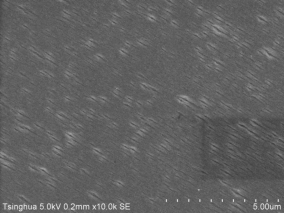
\includegraphics[width=.35\textwidth]{ch05-3_Layers_SEM(a).pdf}
	} 
	\subfigure[] {
		\label{fig:LayersSEM_b}
		\includegraphics[width=.35\textwidth]{ch05-3_Layers_SEM(b).pdf}
	} 
	\subfigure[] {
		\label{fig:LayersSEM_c}
		\includegraphics[width=.35\textwidth]{ch05-3_Layers_SEM(c).pdf}
	}
	\subfigure[] {
		\label{fig:LayersSEM_d}
		\includegraphics[width=.35\textwidth]{ch05-3_Layers_SEM(d).pdf}
	}  
	\caption{腐蚀坑的SEM测试图}
	\label{fig:LayersSEM}
\end{figure}

插入单层量子点作位错阻挡层的样品,腐蚀坑测试失败,致使SEM测试图看不到坑的存在,但是从其他图中可以推测,单层量子点作位错阻挡层效果并不好,还会有大量位错产生。三层量子点和五层量子点做位错阻挡层,对位错都有一定的阻挡作用,可以看到与无位错阻挡层的样品相比,腐蚀坑数量明显减少。其中样品A1的腐蚀坑密度达108 cm-2,A3的腐蚀坑密度为3×107 cm-2, A4的腐蚀坑密度为3×106 cm-2。该结果表明,多层量子点位错阻挡层对位错有一定的阻挡作用,而且量子点层数越多位错阻挡效果越好。
我们对A4样品做了进一步的界面TEM测试,测试结果如图\ref{fig:5LayerTEM}所示

\begin{figure}[ht]
	\centering
	\includegraphics[width=0.4\textwidth]{ch05-3_5Layer_TEM.pdf}
	\caption{界面TEM测试}
	\label{fig:5LayerTEM}
\end{figure}

由图可以看出,位错线在穿过量子点层的时候被阻挡,致使其弯曲不再向上穿透,该结果表明,量子点位错阻挡层对穿透位错有一定的阻挡作用,能够降低外延片表面穿透位错密度。
为了进一步研究大岛团簇对外延片表面穿透位错的影响,我们比较了每层量子点生长时间为65s和70s的三层量子点位错阻挡层的外延片样品。表\ref{tab:TimeXDR}是对两个样片的XRD测试结果

\begin{table*}[htbp] 
	\centering
	\caption{\label{tab:TimeXDR}不同生长时间XDR测试结果}  
	\begin{tabular}{m{.15\textwidth}<{\centering}m{.35\textwidth}<{\centering}m{.35\textwidth}<{\centering}}  
		\toprule
			Sample no. & Growth time of every layer QDs & DCXRD FWHM (arcsec) \\
		\midrule 
			A1 & 65s & 164 \\
			A2 & 70s & 163 \\
		\bottomrule
	\end{tabular}
\end{table*}

从两者的XRD半高宽结果来看,两者半高宽基本相同,进一步验证了插入量子点位错阻挡层之后,用XRD对样品进行测试的结果基本相同,由于XRD测试精度等因素的影响导致XRD不能准确的测量这些样品晶体质量的变化。为了进一步比较我们对两者进行了腐蚀坑的测试。两个样品的SEM测试结果,如图\ref{fig:SpaceSEM}所示

\begin{figure}[ht]
	\centering
	\subfigure[] {
		\label{fig:SpaceSEM_a}
		\includegraphics[width=.35\textwidth]{ch05-3_Space_SEM(a).pdf}
	} 
	\subfigure[] {
		\label{fig:SpaceSEM_b}
		\includegraphics[width=.35\textwidth]{ch05-3_Space_SEM(b).pdf}
	} 
	\caption{SpaceSEM(a)\&(b)}
	\label{fig:SpaceSEM}
\end{figure}

由图\ref{fig:SpaceSEM}可以看出,量子点生长时间为65s的样品腐蚀坑密度明显低于生长时间为70s的样品。而之前对两者AFM的测试结果可以看出,A2岛团簇明显多于A1,由此可以看出,多层量子点位错阻挡层可以阻挡穿透位错,但是大岛团簇也能够导致位错的产生,使得外延片表面穿透位错密度增加。因此,使用量子点位错阻挡层降低表面位错密度的关键是在保证量子点密度的前提下,抑制量子点大岛团簇的产生。


% 本章参考文献
\ifx\usechapbib\empty
\bibliographystyle{buptthesis}
\bibliography{bare_thesis}
\fi

%%% Local Variables: 
%%% mode: latex
%%% TeX-master: "bare_thesis"
%%% End: 
